\documentclass[a4paper,12pt]{article}
\usepackage{indentfirst}
\usepackage[T1]{fontenc}
\usepackage{graphicx}
\usepackage{float}
\usepackage{caption}
\graphicspath{{../Imagens/}{Imagens/}}
\renewcommand{\figurename}{Figura}
\captionsetup{
  justification=raggedright,
  singlelinecheck=false,
  labelsep=endash,
  font=small,
  labelfont=bf,
  skip=6pt,
  position=above
}
\newcommand{\fonteelemento}[1]{%
  \par\smallskip
  {\footnotesize\raggedright Fonte: #1.\par}%
}

\begin{document}

\section{Introdu\c{c}\~ao}

\subsection{Contextualiza\c{c}\~ao}

Os dispositivos vest\'iveis combinam aquisi\c{c}\~ao de dados, processamento embarcado e intera\c{c}\~ao com o usu\'ario em plataformas sujeitas a restri\c{c}\~oes de dimens\~oes, mem\'oria, capacidade computacional e consumo de energia. A disponibilidade de microcontroladores com m\'ultiplos perif\'ericos, sensores miniaturizados e interfaces gr\'aficas tornou vi\'avel a constru\c{c}\~ao de sistemas capazes de reunir fun\c{c}\~oes biom\'etricas, ambientais e inerciais em um \'unico dispositivo. Essa integra\c{c}\~ao, entretanto, n\~ao depende apenas da conex\~ao el\'etrica dos componentes: exige uma organiza\c{c}\~ao de software que coordene diferentes protocolos de comunica\c{c}\~ao, taxas de aquisi\c{c}\~ao, requisitos de processamento e mecanismos de apresenta\c{c}\~ao dos dados (SENEVIRATNE et al., 2017; HESTER et al., 2016).

\`A medida que novos sensores s\~ao incorporados, uma aplica\c{c}\~ao organizada de forma monol\'itica tende a concentrar depend\^encias no n\'ucleo do firmware. Nesse cen\'ario, altera\c{c}\~oes em um subsistema podem repercutir nos demais, dispositivos que compartilham um barramento podem interferir entre si e a falha de um componente pode impedir a inicializa\c{c}\~ao de toda a aplica\c{c}\~ao. Em um sistema embarcado com sistema operacional de tempo real, a integra\c{c}\~ao tamb\'em envolve concorr\^encia entre tarefas, sincroniza\c{c}\~ao de recursos e defini\c{c}\~ao de prioridades, aspectos que precisam ser considerados para preservar a responsividade da interface e o acesso ordenado ao hardware (FREERTOS, 2026c; SHA; RAJKUMAR; LEHOCZKY, 1990).

Esses desafios s\~ao particularmente relevantes em uma plataforma vest\'ivel modular multissensor. Al\'em de acomodar dispositivos com transportes distintos, a plataforma deve permitir a evolu\c{c}\~ao do firmware sem exigir a reestrutura\c{c}\~ao do conjunto a cada nova funcionalidade. Tamb\'em \'e desej\'avel que fun\c{c}\~oes independentes permane\c{c}am dispon\'iveis quando um sensor estiver ausente ou apresentar falha.

\subsection{Defini\c{c}\~ao do problema}

O problema abordado consiste em organizar e integrar sensores heterog\^eneos, interface gr\'afica e servi\c{c}os compartilhados em um dispositivo vest\'ivel com recursos limitados, de modo que a inclus\~ao ou a falha de um m\'odulo n\~ao exija altera\c{c}\~oes disseminadas pelo firmware nem comprometa o funcionamento das fun\c{c}\~oes independentes. A plataforma deve, adicionalmente, coordenar o acesso concorrente ao barramento I$^2$C compartilhado e recuperar sua opera\c{c}\~ao ap\'os falhas de comunica\c{c}\~ao.

Diante desse contexto, formula-se a seguinte quest\~ao de projeto:

\begin{quote}
Como projetar uma plataforma de software modular para um dispositivo vest\'ivel baseado no ESP32-C6, capaz de integrar sensores heterog\^eneos, compartilhar recursos de comunica\c{c}\~ao e permanecer operacional diante da aus\^encia ou falha de m\'odulos?
\end{quote}

A aplica\c{c}\~ao demonstradora re\'une m\'odulos biom\'etricos, ambientais e inerciais, rel\'ogio em tempo real e interface gr\'afica sens\'ivel ao toque. A Figura~\ref{fig:plataforma-aplicacao} diferencia essa instancia\c{c}\~ao da base arquitetural reutiliz\'avel.


\begin{figure}[H]
\centering
\caption{Rela\c{c}\~ao entre a plataforma modular e a aplica\c{c}\~ao demonstradora}
\label{fig:plataforma-aplicacao}
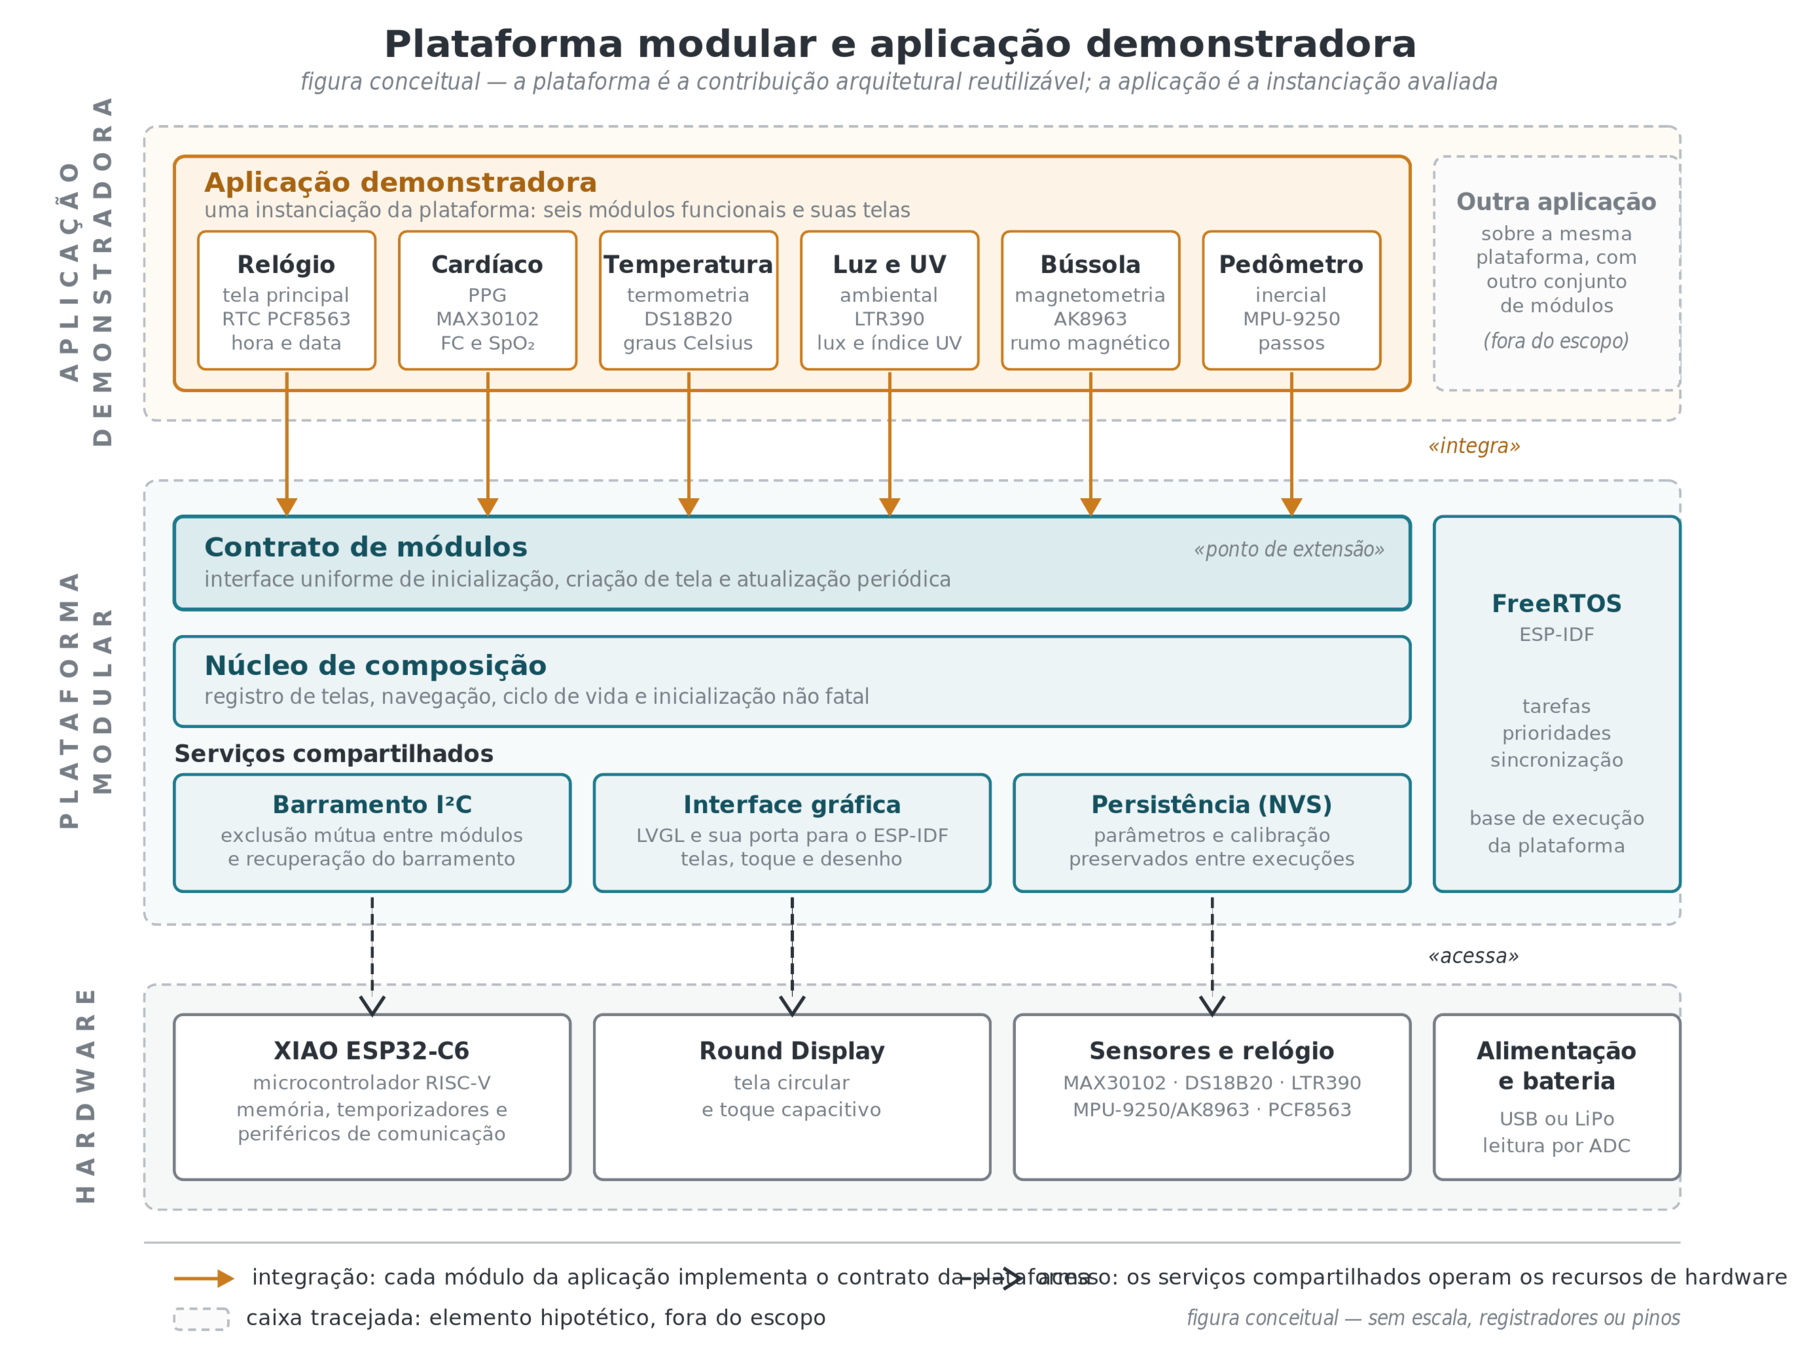
\includegraphics[width=0.96\textwidth]{Diagramas/teoricas/plataforma_aplicacao.png}
\fonteelemento{Elaborado pelo autor}
\end{figure}

\subsection{Objetivo geral}

Projetar e implementar uma plataforma vest\'ivel modular multissensor baseada no XIAO ESP32-C6, capaz de integrar sensores heterog\^eneos, interface gr\'afica e servi\c{c}os compartilhados, verificando estruturalmente sua extensibilidade e observando seu comportamento diante da aus\^encia de m\'odulos.

\subsection{Objetivos espec\'ificos}

Para alcan\c{c}ar o objetivo geral, s\~ao estabelecidos os seguintes objetivos espec\'ificos:

\begin{itemize}
    \item definir uma arquitetura modular para sensores e telas;
    \item estabelecer um contrato uniforme para inicializa\c{c}\~ao dos m\'odulos, cria\c{c}\~ao das telas e acesso \`as funcionalidades;
    \item implementar servi\c{c}os compartilhados de comunica\c{c}\~ao, interface gr\'afica e concorr\^encia;
    \item integrar m\'odulos biom\'etricos, ambientais e inerciais \`a aplica\c{c}\~ao demonstradora;
    \item implementar inicializa\c{c}\~ao n\~ao fatal, de modo que a plataforma possa operar com um subconjunto dos sensores;
    \item coordenar o acesso ao barramento I$^2$C compartilhado e implementar sua recupera\c{c}\~ao ap\'os falhas de comunica\c{c}\~ao;
    \item demonstrar a inclus\~ao de m\'odulos com impacto restrito sobre o n\'ucleo e sobre os m\'odulos existentes;
    \item avaliar o acoplamento, a extensibilidade, o uso est\'atico de mem\'oria e, dentro do escopo experimental, a estabilidade e os mecanismos de robustez da plataforma;
    \item realizar testes funcionais dos m\'odulos integrados; e
    \item produzir documenta\c{c}\~ao t\'ecnica que permita compreender e reproduzir as decis\~oes de arquitetura e integra\c{c}\~ao.
\end{itemize}

\subsection{Justificativa}

A relev\^ancia t\'ecnica do trabalho decorre do tratamento conjunto de problemas que surgem na integra\c{c}\~ao de um sistema embarcado multissensor. A coexist\^encia de dispositivos no mesmo barramento, a execu\c{c}\~ao concorrente de tarefas de aquisi\c{c}\~ao e interface, as diferen\c{c}as entre protocolos e a necessidade de preservar fun\c{c}\~oes independentes diante de falhas exigem decis\~oes que ultrapassam a implementa\c{c}\~ao isolada de drivers. Uma arquitetura com contrato uniforme, servi\c{c}os compartilhados e separa\c{c}\~ao entre n\'ucleo, servi\c{c}os, drivers e m\'odulos oferece uma base para controlar essas depend\^encias e tornar expl\'icitas as responsabilidades de cada parte (PARNAS, 1972; BASS; CLEMENTS; KAZMAN, 2021).

No \^ambito acad\^emico, o trabalho permite discutir a aplica\c{c}\~ao de conceitos de modularidade, extensibilidade, concorr\^encia e toler\^ancia a falhas em uma plataforma embarcada concreta. A escolha do ESP-IDF e do FreeRTOS fornece acesso aos mecanismos de tarefas, prioridades, sincroniza\c{c}\~ao, perif\'ericos e diagn\'ostico empregados na implementa\c{c}\~ao.

Do ponto de vista pr\'atico, a plataforma re\'une m\'odulos com caracter\'isticas distintas: o MAX30102 para fotopletismografia e estimativas de frequ\^encia card\'iaca e SpO$_2$; o DS18B20 para temperatura; o LTR390 para ilumin\^ancia e \'indice UV; e o conjunto MPU-9250/AK8963 para b\'ussola e pedometria. O rel\'ogio em tempo real PCF8563 e a interface gr\'afica no display circular completam a aplica\c{c}\~ao demonstradora. A diversidade desses subsistemas permite observar problemas de integra\c{c}\~ao que n\~ao aparecem quando cada sensor \'e operado isoladamente.

\subsection{Contribui\c{c}\~oes do trabalho}

A contribui\c{c}\~ao principal \'e a arquitetura da plataforma, estruturada em m\'odulos autocontidos e em um contrato uniforme de integra\c{c}\~ao com o n\'ucleo e a interface. A implementa\c{c}\~ao inclui tarefas independentes de aquisi\c{c}\~ao, ativa\c{c}\~ao da aquisi\c{c}\~ao conforme a tela exibida, registro de telas e fun\c{c}\~oes de atualiza\c{c}\~ao, inicializa\c{c}\~ao n\~ao fatal e opera\c{c}\~ao com os m\'odulos dispon\'iveis.

Tamb\'em integram a contribui\c{c}\~ao o tratamento do barramento I$^2$C compartilhado por meio de exclus\~ao m\'utua com heran\c{c}a de prioridade, a recupera\c{c}\~ao p\'os-NACK e o scanner de dispositivos executado na inicializa\c{c}\~ao. Complementam a plataforma o uso pragm\'atico de drivers pr\'oprios e componentes oficiais, bem como a persist\^encia da calibra\c{c}\~ao da b\'ussola em mem\'oria n\~ao vol\'atil.

\subsection{Delimita\c{c}\~ao do escopo}

O escopo compreende o projeto da arquitetura, sua implementa\c{c}\~ao em C com ESP-IDF 5.5.1 e FreeRTOS em configura\c{c}\~ao unicore, a integra\c{c}\~ao dos sensores e da interface gr\'afica e a avalia\c{c}\~ao funcional e arquitetural da plataforma. A avalia\c{c}\~ao arquitetural abrangeu extensibilidade e acoplamento por an\'alise est\'atica, mem\'oria global da configura\c{c}\~ao integrada e ensaios qualitativos de inicializa\c{c}\~ao e opera\c{c}\~ao com sensores ausentes. CPU e heap por cen\'ario, mem\'oria incremental, falha I$^2$C induzida, s\'erie de boot e ensaio prolongado completo foram delimitados fora do escopo experimental desta vers\~ao.

O dispositivo n\~ao possui finalidade m\'edica. Os valores de frequ\^encia card\'iaca e a estimativa de SpO$_2$ destinam-se a testes funcionais, sem valida\c{c}\~ao cl\'inica ou certifica\c{c}\~ao para diagn\'ostico. Tamb\'em n\~ao fazem parte do estado implementado a compensa\c{c}\~ao de inclina\c{c}\~ao da b\'ussola, a persist\^encia do ped\^ometro, o gerenciamento avan\c{c}ado de energia e a conectividade sem fio. A placa prot\'otipo autoral e o inv\'olucro impresso em 3D foram realizados, embora sua caracteriza\c{c}\~ao mec\^anica e ambiental n\~ao tenha integrado os ensaios.

\subsection{Organiza\c{c}\~ao do documento}

Al\'em desta Introdu\c{c}\~ao, o trabalho est\'a organizado em cinco partes principais. A Fundamenta\c{c}\~ao Te\'orica apresenta os conceitos necess\'arios \`a compreens\~ao dos dispositivos vest\'iveis, da arquitetura modular, do sistema operacional de tempo real, dos protocolos de comunica\c{c}\~ao, da interface gr\'afica e dos princ\'ipios de opera\c{c}\~ao dos sensores. Materiais e M\'etodos descreve a plataforma f\'isica e de software, o m\'etodo de desenvolvimento, os requisitos, os crit\'erios de aceita\c{c}\~ao e os procedimentos experimentais.

Desenvolvimento e Implementa\c{c}\~ao detalha a arquitetura de hardware e software, o contrato dos m\'odulos, o modelo de concorr\^encia, os mecanismos de robustez e a implementa\c{c}\~ao dos subsistemas. Resultados e Discuss\~ao re\'une as evid\^encias obtidas nos ensaios, interpreta o comportamento da plataforma e explicita suas limita\c{c}\~oes. Por fim, as Conclus\~oes retomam o problema e os objetivos, sintetizam as contribui\c{c}\~oes sustentadas pelos resultados e indicam possibilidades de continuidade. Refer\^encias, ap\^endices e eventuais anexos complementam o documento.

\end{document}
